\documentclass{book}
\usepackage[utf8]{inputenc}

\usepackage{graphicx}
\title{Computational Neuroscience}
\author{Huynh Xuan Phung - Coursera}
\date{ }
\usepackage{color}   %May be necessary if you want to color links
\usepackage{hyperref}
\hypersetup{
    colorlinks=true, %set true if you want colored links
    linktoc=all,     %set to all if you want both sections and subsections linked
    linkcolor=blue,  %choose some color if you want links to stand out
} 
\begin{document}
 
\maketitle
 
\tableofcontents

\chapter{Introduction and Basic Neurobiology}

\section{Computational Neuroscience}
\subsection{Descriptive Models}

What is Computational Neuroscience?
Computational Neuro-science provides tools and methods for "characterizing what nervous systems do, determining how they function, and understanding why they operate in particular ways"

Descriptive Models (What)

Mechanistic Models (How)

Interpretive Models (Why)

Frequency of spikes = f(Light bar's orientation). 

"receptive field" of a neuron is the particular orientation of a bar of light that produces the best response. That is maximizes f(Light Bar's orientation) (45 degree is maximize).

A greater response corresponds to more frequent "spikes" (or action potentials)

Receptive Field: is specific properties of a sensory stimulus that generate a strong response from the cell

Examples:
\begin{itemize}
	\item {Spot of light that turns on at a particular location on the retina}
	\item{Bar of light that turns on at a particular orientation and location on the retina}
\end{itemize} 

\subsection{Descriptive Model of Receptive Fields}
\begin{figure}[h]
\centering
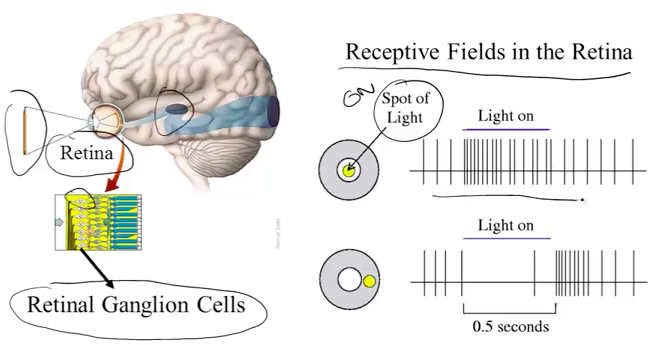
\includegraphics[width=0.7\linewidth]{figures/ReceptiveField_Retina}
\caption{}
\label{fig:receptivefieldretina}
\end{figure}

Center-Surround Receptive Fields on the Retina

--- On-Center Off-Surround: center of the small patch of retina associated with the cell

The ON-Center/ Off-Surround receptive field can be thought of as a filter. The filter causes activation with stimuli concentrates on the center of the receptive field and depressing activation with stimuli which are concentrated in the surround.

\subsection{Descriptive models: Cortical Receptive Fields}
\begin{figure}[h]
\centering
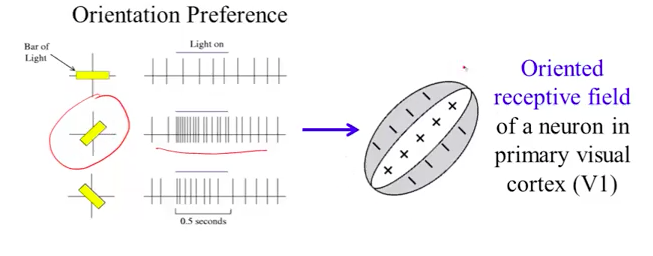
\includegraphics[width=0.7\linewidth]{figures/ReceptiveField_V1}
\caption{}
\label{fig:receptivefieldv1}
\end{figure}

Oriented receptive field of a neuron in primary visual cortex (V1)



\subsection{Mechanistic and Interpretive Models}

Mechanistic Model of Receptive File

\begin{figure}[h]
\centering
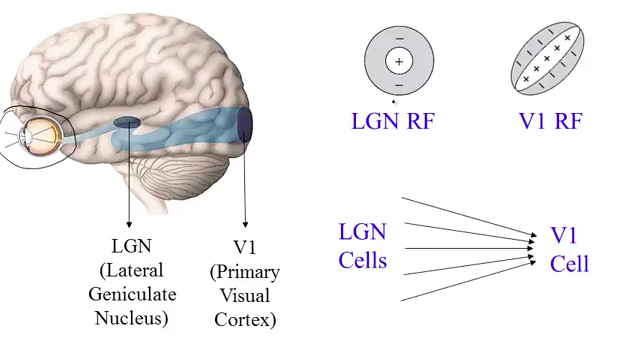
\includegraphics[width=0.7\linewidth]{figures/mechanistic_v1}
\caption{}
\label{fig:mechanisticv1}
\end{figure}

Number of LGN cells converges to one V1 cell: arrange LGN to one V1 cell

\begin{figure}[h]
\centering
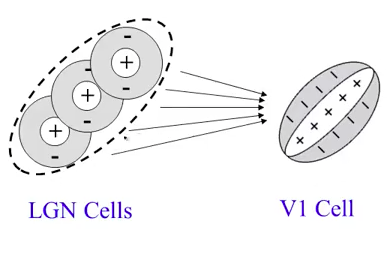
\includegraphics[width=0.7\linewidth]{figures/V1Cell}
\caption{}
\label{fig:v1cell}
\end{figure}

\subsection{Interpretive Model of Receptive Fields}

Why do they have orientation, or selected of black and white dot?

Efficient Coding Hypothesis: Suppose the goal is to represent images as faithfully ans efficiently as possible using neurons with receptive fields $RF_1,RF_2$, etc 

Given image I, we can reconstruct I using neural response $r_1,r_2$ ..

$ \hat{I} = \sum_{i} RF_i r_i$

Idea: What are the $RF_i$ that minimize the total squared pixelwise errors between I and $\hat{I}$ and are as independent as possible?


Start out with random $RF_i$, and run your efficient coding algorithm on natural image patches. efficient coding: Sparse coding/ ICA/ Predictive coding.



\section{The Electrical Personality of Neurons}

\section{Making Connections: Synapses}

\section{Time to Network: Brain Areas and Their Function}

 

 
\end{document}